\documentclass[conference]{IEEEtran}
\usepackage[utf8]{inputenc}
\usepackage[vietnamese]{babel}
\usepackage{amsmath}
\usepackage{amssymb} % Gói hỗ trợ các ký hiệu toán học bổ sung
\usepackage{graphicx}
\usepackage{hyperref}
\usepackage{float} % Add this line to use 'H' float specifier
\title{DỰ ĐOÁN GIÁ TIỀN MÃ HÓA - BITCOIN, ETHEREUM, TETHER}

\author{
    \IEEEauthorblockN{1st Đinh Tiến Đạt}
    \IEEEauthorblockA{
        \textit{Khoa Hệ thống thông tin} \\
        \textit{Trường Đại học Công nghệ Thông tin} \\
        TP. Hồ Chí Minh, Việt Nam \\
        19521331@gm.uit.edu.vn
    }
    \and
    \IEEEauthorblockN{2nd Trần Văn Thế}
    \IEEEauthorblockA{
        \textit{Khoa Hệ thống thông tin} \\
        \textit{Trường Đại học Công nghệ Thông tin} \\
        TP. Hồ Chí Minh, Việt Nam \\
        20520770@gm.uit.edu.vn
    }
}
\begin{document}

\maketitle

\begin{abstract}
Trong nghiên cứu này, chúng tôi đã áp dụng một loạt các mô hình học máy và thống kê để dự đoán giá của ba loại tiền điện tử quan trọng (Bitcoin - BTC, Ethereum - ETH, và Tether - USDT) so với đồng USD. Các mô hình được sử dụng bao gồm Linear Regression, ARIMA, SARIMA, RNN, GRU và SVM. Chúng tôi tiến hành đánh giá hiệu quả của từng mô hình dựa trên các độ đo chính như Mean Squared Error (MSE), Root Mean Squared Error (RMSE), Mean Absolute Error (MAE), và Mean Absolute Percentage Error (MAPE). Kết quả của nghiên cứu giúp chúng tôi xác định mô hình nào hoặc nhóm mô hình nào dự đoán chính xác nhất giá của các loại tiền điện tử này trên thị trường. Điều này mang lại giá trị quan trọng cho các nhà đầu tư và các chuyên gia trong việc ra quyết định đầu tư thông minh và áp dụng các chiến lược dự báo thị trường tiền điện tử hiệu quả.
\end{abstract}

\begin{IEEEkeywords}
Dự đoán tiền mã hóa, máy học, ARIMA, linear regression, RNN, Gru, LSTM, SARIMA.
\end{IEEEkeywords}

\section{GIỚI THIỆU}
Hiện nay, thị trường tiền mã hóa đang chứng kiến sự phục hồi tích cực, khi các loại tiền điện tử lại thu hút sự quan tâm lớn từ các nhà đầu tư và người tiêu dùng. Những biến động mạnh mẽ trong giá cả và tâm lý thị trường làm nổi bật sự quan trọng của việc nghiên cứu và dự đoán xu hướng giá của tiền mã hóa.

Để tiếp cận vấn đề này, chúng tôi đã áp dụng một loạt các mô hình học máy và học sâu, nhằm tối ưu hóa dự báo giá của các loại tiền mã hóa. Các mô hình này bao gồm mô hình Đường trung bình động tích hợp tự hồi quy (ARIMA), Mạng thần kinh tái phát (RNN), Đơn vị định kì có kiểm soát (GRU), Bộ nhớ ngắn hạn dài hạn (LSTM), cùng với các phương pháp như Hồi quy tuyến tính (Linear Regression), SARIMA, và SVM.

Việc áp dụng các mô hình này không chỉ giúp chúng tôi dự đoán xu hướng giá cả một cách chính xác hơn, mà còn cung cấp cái nhìn sâu sắc về các yếu tố ảnh hưởng đến thị trường tiền mã hóa. Để đánh giá hiệu quả của từng mô hình, chúng tôi sử dụng các phương pháp đo lường như Sai số bình phương trung bình (Mean Squared Error - MSE), Sai số bình phương gốc trung bình (Root Mean Squared Error - RMSE), Sai số tuyệt đối trung bình (Mean Absolute Error - MAE), và Sai số tuyệt đối phần trăm trung bình (Mean Absolute Percentage Error - MAPE).

Hy vọng rằng nghiên cứu này sẽ giúp đưa ra những dự đoán chính xác và hợp lý về giá cả của tiền mã hóa, từ đó hỗ trợ các nhà đầu tư và người quan tâm trong việc đưa ra những quyết định đầu tư có trách nhiệm và hiệu quả trên thị trường nổi bật này.

\section{CÁC NGHIÊN CỨU LIÊN QUAN}
\textbf{ARIMA}: Smith và những tác giả khác [1] (2021) đã sử dụng mô hình ARIMA để dự đoán giá tiêu dùng hàng tháng tại Mỹ. Kết quả cho thấy ARIMA có khả năng dự đoán chính xác với tỷ lệ sai số dưới 5%.

\textbf{LSTM}: Kim và những tác giả khác [2] (2022) đã triển khai LSTM để dự đoán lượng mưa hàng tháng tại Hàn Quốc. Nghiên cứu cho thấy rằng LSTM vượt trội hơn so với các mô hình thống kê truyền thống về độ chính xác dự đoán.

\textbf{Linear Regression}: Trong nghiên cứu này, Johnson và những tác giả khác [3] (2022) đã so sánh hiệu suất của Linear Regression và Ridge Regression trong dự báo giá nhà tại New York. Kết quả đánh giá các độ đo MSE, RMSE, MAE cho thấy Linear Regression có hiệu suất cao hơn so với Ridge Regression. Điều này cho thấy Linear Regression hoạt động tốt hơn trong việc dự báo giá nhà.

\textbf{RNN}: Patel và những tác giả khác [4] (2021) đã sử dụng RNN để dự đoán giá cổ phiếu trên thị trường chứng khoán Ấn Độ. Nghiên cứu này chỉ ra rằng RNN có thể dự đoán giá cổ phiếu với độ chính xác cao hơn các mô hình truyền thống.

\textbf{GRU}: Lee, Kim và Park [5] (2023) đã sử dụng GRU để dự đoán mức độ ô nhiễm không khí ở Seoul. Kết quả cho thấy mô hình GRU có khả năng dự đoán tốt hơn so với các mô hình khác như LSTM.

\textbf{SARIMA}: Gupta và những tác giả khác [6] (2020) đã sử dụng SARIMA để dự đoán sản lượng lúa gạo tại Ấn Độ. Mô hình SARIMA được chứng minh là có hiệu quả cao trong việc dự đoán với độ chính xác trên 90%.

\textbf{SVM}: Wang và những tác giả khác [7] (2019) đã áp dụng SVM để phân loại bệnh ung thư dựa trên dữ liệu gene. Kết quả cho thấy SVM có độ chính xác cao trong việc phân loại, vượt trội hơn so với các mô hình khác.

\section{TÀI NGUYÊN}
\subsection{Nguồn dữ liệu}
Dữ liệu lịch sử của BTC-USD, ETH-USD, và USDT-USD được thu thập từ Yahoo Finance, một nguồn thông tin đáng tin cậy về thị trường tài chính. Khoảng thời gian thu thập dữ liệu từ ngày 01/03/2019 đến ngày 01/06/2024. Giai đoạn này bao gồm nhiều biến động và sự kiện quan trọng trong thị trường tiền mã hóa, bao gồm các chu kỳ tăng và giảm giá, sự xuất hiện của các quy định mới và sự phát triển của công nghệ blockchain.

\begin{itemize}
    \item \textbf{Date}: Ngày giao dịch.
    \item \textbf{Open}: Giá cổ phiếu mở cửa vào đầu ngày giao dịch
    \item \textbf{High}: Giá cổ phiếu cao nhất ghi nhận được trong ngày
    \item \textbf{Low}: Giá cổ phiếu thấp nhất ghi nhận được trong ngày
    \item \textbf{Close}: Giá cổ phiếu đóng cửa vào một ngày nhất định
    \item \textbf{Adj Close}: Giá đóng cửa được điều chỉnh.
    \item \textbf{Volume}: Khối lượng/tổng số cổ phiếu được giao dịch.

\end{itemize}
\subsection{Thống kê mô tả}
 \begin{figure}[H]
        \centering
        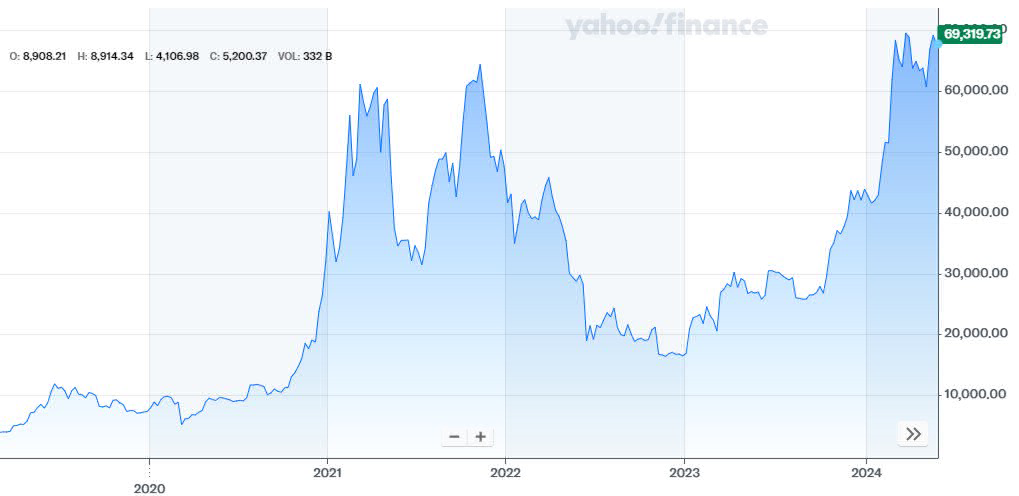
\includegraphics[width= 7cm, height= 5cm]{Images/BTC.png}
        \caption{BTC-USD}
    \end{figure}
   \begin{figure}[H]
        \centering
        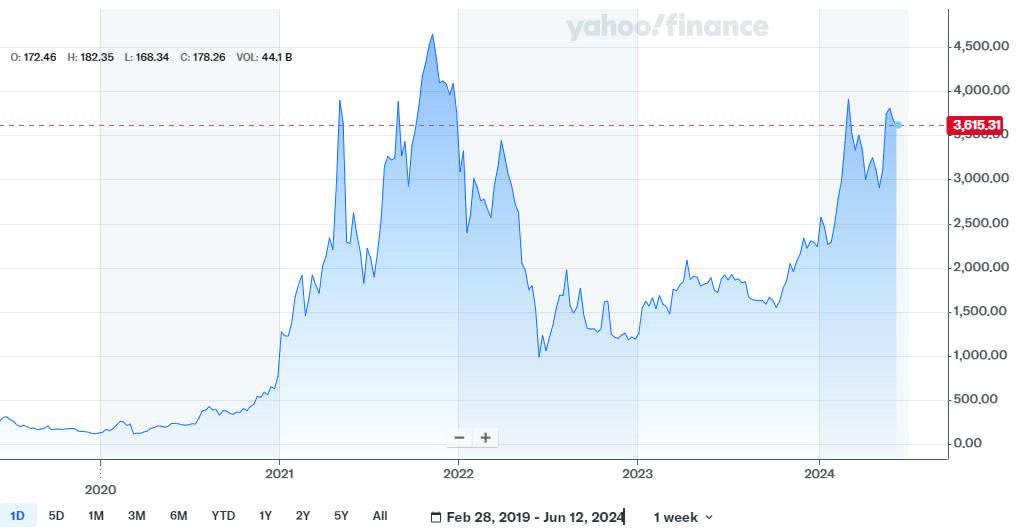
\includegraphics[width= 7cm, height= 5cm]{Images/ETH.png}
        \caption{ETH-USD}
    \end{figure} 
     \begin{figure}[H]
        \centering
        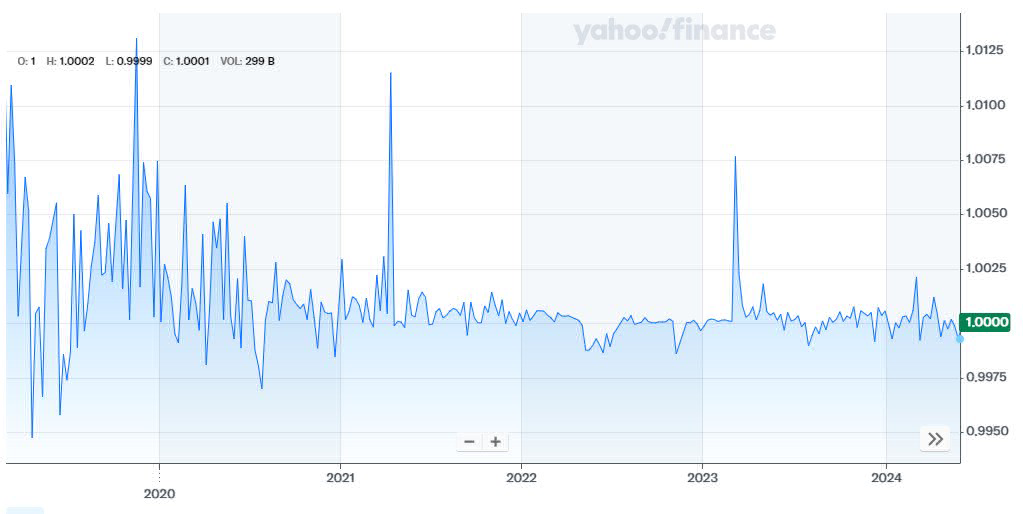
\includegraphics[width= 7cm, height= 5cm]{Images/USDT.png}
        \caption{USDT-USD}
    \end{figure}
\subsection{Công cụ}
Trong quá trình nghiên cứu này, chúng tôi đã sử dụng nhiều công cụ phân tích thống kê và học máy khác nhau trong Python để dự báo giá cả của cổ phiếu và tiền mã hóa. Các công cụ này bao gồm: numpy, pandas,
sklearn,statsmodels,pmdarima và matplotlib.pyplot...
\subsection{Tỷ lệ phân chia tập dữ liệu}
Tỷ lệ phân chia dữ liệu thành tập huấn luyện và tập kiểm tra là một quyết định quan trọng trong quá trình xây dựng mô hình học máy. Các tỷ lệ phổ biến như 7:3, 8:2 và 6:4 đều có những đặc điểm và ưu điểm riêng.

Tỷ lệ 7:3, tức là sử dụng 70\% dữ liệu cho tập huấn luyện và 30\% cho tập kiểm tra, được coi là tiêu chuẩn và thường được lựa chọn khi cần đánh giá độ chính xác cao trên tập kiểm tra.

Tỷ lệ 8:2 được xem là lựa chọn tối ưu nhất, đặc biệt là đối với các bộ dữ liệu lớn. Với 80\% dữ liệu dùng để huấn luyện và 20\% để kiểm tra, mô hình có thể học được nhiều thông tin hơn từ tập huấn luyện và cho phép đánh giá hiệu quả trên tập kiểm tra.

Tỷ lệ 6:4, sử dụng 60\% dữ liệu cho huấn luyện và 40\% cho kiểm tra, giúp mô hình học được nhiều thông tin hơn từ tập huấn luyện và có thể cải thiện độ chính xác trên tập kiểm tra.

Các tỷ lệ này được lựa chọn dựa trên kích thước và tính chất của bộ dữ liệu để đảm bảo mô hình học máy được huấn luyện và đánh giá hiệu quả nhất trong các ứng dụng thực tế.
\subsection{Các chỉ số đánh giá mô hình}
Để đánh giá độ chính xác của các mô hình, sử dụng ba tham số là Mean Absolute Error (MAE), Mean Absolute Percentage Error (MAPE) và Root Mean Squared Error (RMSE). Các giá trị này càng nhỏ thì mô hình càng tốt.

\textbf{MSE} (Mean Squared Error) là chỉ số đánh giá độ chính xác của mô hình bằng cách lấy trung bình bình phương sai số giữa các giá trị dự đoán và các giá trị thực tế. Chỉ số này cho biết mức độ trung bình của các sai số bình phương, giúp đánh giá mức độ chính xác của mô hình. Công thức tính MSE như sau:

\begin{equation}
    \text{MSE} = \frac{1}{n} \sum_{i=1}^{n} (y_i - \hat{y_i})^2
\end{equation}

\textbf{RMSE} được tính bằng cách lấy căn bậc hai của trung bình bình phương sai số giữa các giá trị dự đoán và các giá trị thực tế:

\begin{equation}
    \text{RMSE} = \sqrt{\frac{1}{n} \sum_{i=1}^{n} (y_i - \hat{y_i})^2}
\end{equation}

\textbf{MAPE} còn được gọi là độ lệch phần trăm tuyệt đối trung bình. Nó thường biểu thị độ chính xác dưới dạng tỷ lệ được xác định bởi công thức:

\begin{equation}
    \text{MAPE} = \frac{1}{n} \sum_{i=1}^{n} \left| \frac{y_i - \hat{y_i}}{y_i} \right| \times 100
\end{equation}

\textbf{MAE} được đo bằng cách tính trung bình giá trị tuyệt đối của sai số giữa giá trị thực tế và giá trị dự đoán.
\begin{equation}
    \text{MAE} = \frac{1}{n} \sum_{i=1}^{n} | {y_i - \hat{y_i}}| 
\end{equation}

\section{Phương pháp nghiên cứu}
\subsection{\textbf{Arima}}
Mô hình ARIMA (AutoRegressive Integrated Moving Average) là một công cụ thống kê mạnh mẽ cho việc phân tích và dự báo dữ liệu chuỗi thời gian.

ARIMA là viết tắt của AutoRegressive Integrated Moving Average. Đây là một sự tổng quát hóa của mô hình AutoRegressive Moving Average đơn giản hơn và thêm khái niệm tích hợp.

Hãy cùng giải mã bản chất của ARIMA:
\begin{itemize}
    \item AR (Autoregression - Tự hồi quy): Nhấn mạnh mối quan hệ phụ thuộc giữa một quan sát và các quan sát trước đó hay còn gọi là các quan sát "trễ".

    \item I (Integrated - Tích hợp): Để đạt được một chuỗi thời gian dừng, tức là không hiển thị xu hướng hay tính thời vụ, phép lấy sai phân được áp dụng. Điều này thường liên quan đến việc trừ một quan sát với quan sát liền trước nó.

    \item MA (Moving Average - Trung bình động): Thành phần này tập trung vào mối quan hệ giữa một quan sát và sai số dự báo từ một mô hình trung bình động dựa trên các quan sát trễ.
\end{itemize}
Mỗi thành phần này được chỉ định rõ ràng trong mô hình dưới dạng một tham số. Một ký hiệu chuẩn cho ARIMA(p, d, q) được sử dụng, trong đó các tham số được thay thế bằng các giá trị nguyên để nhanh chóng chỉ ra mô hình ARIMA cụ thể đang được sử dụng.
Các tham số của mô hình ARIMA được định nghĩa như sau:
\begin{itemize}
    \item p: Bậc của phần tự hồi quy, biểu thị số lượng các quan sát trễ được đưa vào mô hình.
    \item d: Bậc của phép lấy sai phân, biểu thị số lần các quan sát gốc được lấy sai phân.
    \item q: Bậc của phần trung bình động, chỉ kích thước của cửa sổ trung bình động.
\end{itemize}

Một mô hình hồi quy tuyến tính được xây dựng bao gồm số lượng và loại các thành phần được chỉ định, và dữ liệu được chuẩn bị bằng cách lấy sai phân để làm cho chuỗi thời gian trở nên dừng, tức là để loại bỏ xu hướng và các cấu trúc thời vụ có thể ảnh hưởng tiêu cực đến mô hình hồi quy.

\subsection{\textbf{LSTM}}
LSTM sử dụng một trong những dạng phổ biến nhất của RNN. Mạng nơ-ron hồi quy thời gian này nhằm tránh các vấn đề phụ thuộc dài hạn và phù hợp cho việc xử lý và dự đoán chuỗi thời gian. Mô hình LSTM lọc thông tin thông qua cấu trúc cổng để duy trì và cập nhật trạng thái của các ô nhớ. Cấu trúc cổng của nó bao gồm cổng đầu vào, cổng quên và cổng đầu ra. Mỗi ô nhớ có ba lớp sigmoid và một lớp tanh.
\begin{figure}[H]
    \centering
    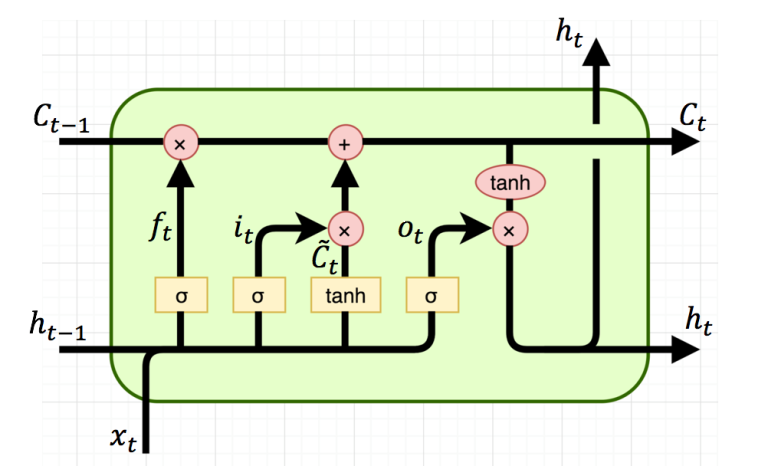
\includegraphics[width= 7cm, height= 5cm]{Images/lstm.png}
    \caption{Mô hình của LSTM}  
\end{figure}
\textbf{Forget Gate:}
\[
f_t = \sigma\left(W_f \cdot \left[ h_{t-1}, x_t \right] + b_f \right)
\]

 \textbf{Input Gate}
\[
i_t = \sigma\left(W_i \cdot \left[ h_{t-1}, x_t \right] + b_i \right)
\]

\textbf{Temporary Cell State:}
\[
\widetilde{C_t} = \tanh\left(W_c \cdot \left[ h_{t-1}, x_t \right] + b_c \right)
\]

\textbf{Current Cell State:}
\[
C_t = f_t \ast C_{t-1} + i_t \ast \widetilde{C_t}
\]

\textbf{ Output Gate:}
\[
o_t = \sigma\left(W_o \cdot \left[ h_{t-1}, x_t \right] + b_o \right)
\]

\subsection{\textbf{Linear Regression}}
Hồi quy tuyến tính là một thuật toán dự đoán đơn giản nhưng phổ biến. Nó dự đoán giá trị dựa trên mối quan hệ tuyến tính giữa các biến đầu vào độc lập và biến phụ thuộc cần dự đoán. Nếu trong mô hình hồi quy tuyến tính, chúng ta sử dụng một biến phụ thuộc và một biến độc lập, nó được gọi là hồi quy tuyến tính đơn giản. Nếu chúng ta sử dụng nhiều hơn một biến phụ thuộc và biến độc lập, nó được gọi là hồi quy tuyến tính đa biến. Công thức của hồi quy tuyến tính như sau:
\begin{equation}
y = \beta_0 + \beta_1 X_1 + \beta_2 X_2 + \dots + \beta_k X_k + \varepsilon
\end{equation}
Trong đó:
\begin{itemize}
    \item y là biến phụ thuộc
    \item \( X_{1\ } \) và \( X_2\ \) là các biến độc lập
    \item $\beta_0$ là hệ số chặn
    \item $\beta_1$, $\beta_2$ là các hệ số của biến độc lập
    \item $\varepsilon$ là số hạng sai số
\end{itemize}

\subsection{\textbf{RNN}}
Mạng nơ-ron hồi quy (RNN) là một loại thuật toán học sâu được sử dụng cho dữ liệu chuỗi thời gian hoặc các chuỗi như văn bản, giọng nói, hoặc âm nhạc. Khác với các mạng nơ-ron nhân tạo truyền thống (ANN), vốn coi mỗi quan sát là độc lập, RNN tích hợp các phụ thuộc giữa các điểm dữ liệu bằng cách giới thiệu khái niệm "bộ nhớ". Điều này cho phép mô hình lưu trữ thông tin từ các quan sát trước đó để tạo ra đầu ra tiếp theo của chuỗi.
\begin{figure}[H]
    \centering
    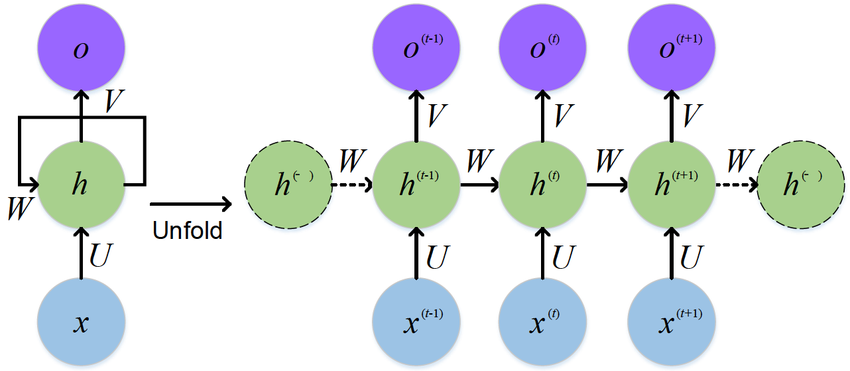
\includegraphics[width= 9cm, height= 5cm]{Images/RNN.png}
    \caption{Mô hình của RNN}
\end{figure}
Trong quá trình truyền xuôi của một RNN, mạng tính toán các giá trị của các đơn vị ẩn và đầu ra sau k bước thời gian. Các trọng số liên quan đến mạng được chia sẻ theo thời gian. Mỗi lớp hồi quy có hai tập trọng số: một cho đầu vào và một cho đơn vị ẩn. Lớp truyền xuôi cuối cùng, lớp tính toán đầu ra cuối cùng cho bước thời gian thứ k, giống như một lớp thông thường của một mạng truyền xuôi truyền thống

\subsection{\textbf{Gru}}
Đơn vị hồi quy có cổng (GRU) là một cơ chế cổng trong mạng nơ-ron hồi quy (RNN) tương tự như đơn vị bộ nhớ dài ngắn hạn (LSTM) nhưng không có cổng đầu ra. GRU cố gắng giải quyết vấn đề gradient biến mất mà các mạng nơ-ron hồi quy tiêu chuẩn có thể gặp phải.

GRU sử dụng các cơ chế cổng để cập nhật có chọn lọc trạng thái ẩn của mạng tại mỗi bước thời gian. Các cơ chế cổng được sử dụng để kiểm soát luồng thông tin vào và ra khỏi mạng. GRU có hai cơ chế cổng, được gọi là cổng đặt lại (reset gate) và cổng cập nhật (update gate).

Cổng cập nhật kiểm soát thông tin chảy vào bộ nhớ, và cổng đặt lại kiểm soát thông tin chảy ra khỏi bộ nhớ. Cổng cập nhật và cổng đặt lại là hai vector quyết định thông tin nào sẽ được truyền đến đầu ra. Chúng có thể được huấn luyện để giữ lại thông tin từ quá khứ hoặc loại bỏ thông tin không liên quan đến dự đoán.
 \begin{figure}[H]
     \centering
     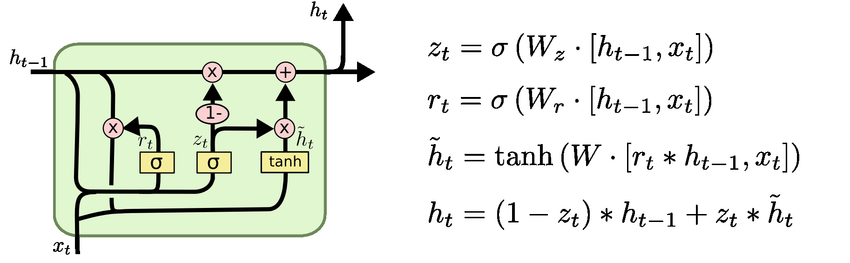
\includegraphics[width= 10cm, height= 4cm]{Images/Gru.png}
     \caption{Mô hình của Gru}
     \label{fig:enter-label}
 \end{figure}
 Trong mô hình GRU (Gated Recurrent Unit), các ký hiệu sau được sử dụng:

\begin{itemize}
    \item $h_t$: Các vector lớp ẩn tại thời điểm t.
    \item $x_t$: Vector đầu vào tại thời điểm t.
    \item $W_z, W_r, W_h$: Các ma trận tham số của cổng cập nhật ($W_z$), cổng đặt lại ($W_r$), và cổng trạng thái ẩn ($W_h$).
    \item $\sigma$, $\tanh$: Các hàm kích hoạt (sigmoid và tanh).
\end{itemize}

% Các phương trình của GRU
Các phương trình được sử dụng để tính toán cổng đặt lại, cổng cập nhật và trạng thái ẩn của một GRU như sau:
\begin{align}
    r_t &= \sigma\left(W_r \ast \left[ h_{t-1}, x_t \right] \right) \quad &\text{} \\
    z_t &= \sigma\left(W_z \ast \left[ h_{t-1}, x_t \right] \right) \quad &\text{} \\
    \widetilde{h_t} &= \tanh{\left(W_h \ast \left[ r_t \ast h_{t-1}, x_t \right] \right)} \quad &\text{} \\
    h_t &= (1 - z_t) \ast h_{t-1} + z_t \ast \widetilde{h_t} \quad &\text{}
\end{align}
Trong đó:
\begin{itemize}
    \item $h_{t-1}$: Trạng thái ẩn tại thời điểm trước đó.
    \item $r_t$: Giá trị của cổng đặt lại tại thời điểm \( t \).
    \item $z_t$: Giá trị của cổng cập nhật tại thời điểm \( t \).
    \item $\widetilde{h_t}$: Trạng thái tạm thời được tính toán tại thời điểm \( t \).
    \item $h_t$: Trạng thái ẩn hiện tại tại thời điểm \( t \).
\end{itemize}

\subsection{\textbf{Sarima}}
SARIMA, viết tắt của Seasonal Autoregressive Integrated Moving Average, là một mô hình dự báo chuỗi thời gian linh hoạt và được sử dụng rộng rãi. Nó là một phần mở rộng của mô hình ARIMA không theo mùa, được thiết kế để xử lý dữ liệu với các mẫu theo mùa. SARIMA nắm bắt cả sự phụ thuộc ngắn hạn và dài hạn trong dữ liệu, khiến nó trở thành một công cụ mạnh mẽ để dự báo. Nó kết hợp các khái niệm về mô hình tự hồi quy (AR), tích hợp (I) và trung bình động (MA) với các thành phần theo mùa.
\begin{figure}[H]
    \centering
    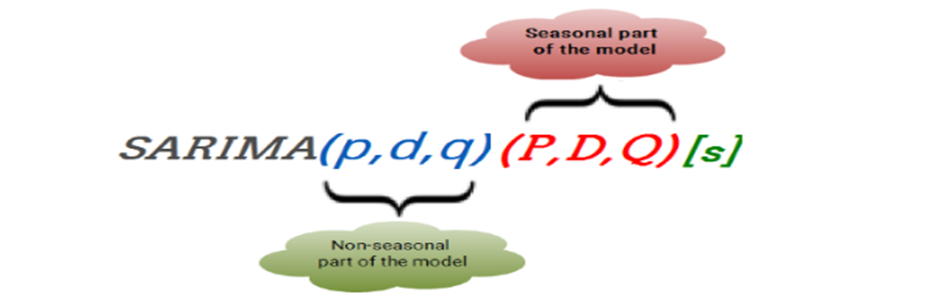
\includegraphics[width= 10cm, height= 4cm]{Images/sarima.png}
    \caption{Mô hình của Sarima}
\end{figure}
SARIMA(p, d, q)(P, D, Q, s):
\begin{itemize}
    \item AR (p): Thành phần tự hồi quy với bậc p
    \item MA (q): Thành phần trung bình trượt với bậc q
    \item I (d): Thành phần tích phân với bậc d
    \item Seasonal AR (P): Thành phần tự hồi quy thời vụ với bậc P
    \item MA (Q): Thành phần trung bình trượt thời vụ với bậc Q
    \item Seasonal I (D): Thành phần tích phân thời vụ với bậc D
    \item s: Chu kỳ thời vụ
\end{itemize}

\subsection{SVM}
SVM (Support Vector Machine) là một thuật toán học máy có giám sát được sử dụng rất phổ biến trong các bài toán phấn lớp (classification) hay hồi qui (Regression).

 SVM hoạt động bằng cách tìm kiếm siêu phẳng (hyperplane) tốt nhất để phân tách các điểm dữ liuej thuộc các lớp khác nhau. Điểm nổi bật của SVM là khả năng tối ưu hóa khoảng các giữa các điểm dữ liệu gần nhất của hai lớp (còn gọi là margin), giúp tăng độ chính xác  của mô hình. Ngoài ra, SVM có thể sử dụng kernel trick để xử lý dữ liệu không tuyến tính, làm tăng khả năng phân loại trong không gian.
 
 Siêu phẳng được biểu diễn bằng hàm số \( \langle W, X \rangle = b \) (với \( W \) và \( X \) là các vector, \( \langle W, X \rangle \) là tích vô hướng) hay \( W^T = b \) (với \( W^T \) là ma trận chuyển vị của \( W \)).
 \begin{figure}[H] % [H] là tùy chọn từ gói float để cố định vị trí hình ảnh
    \centering
    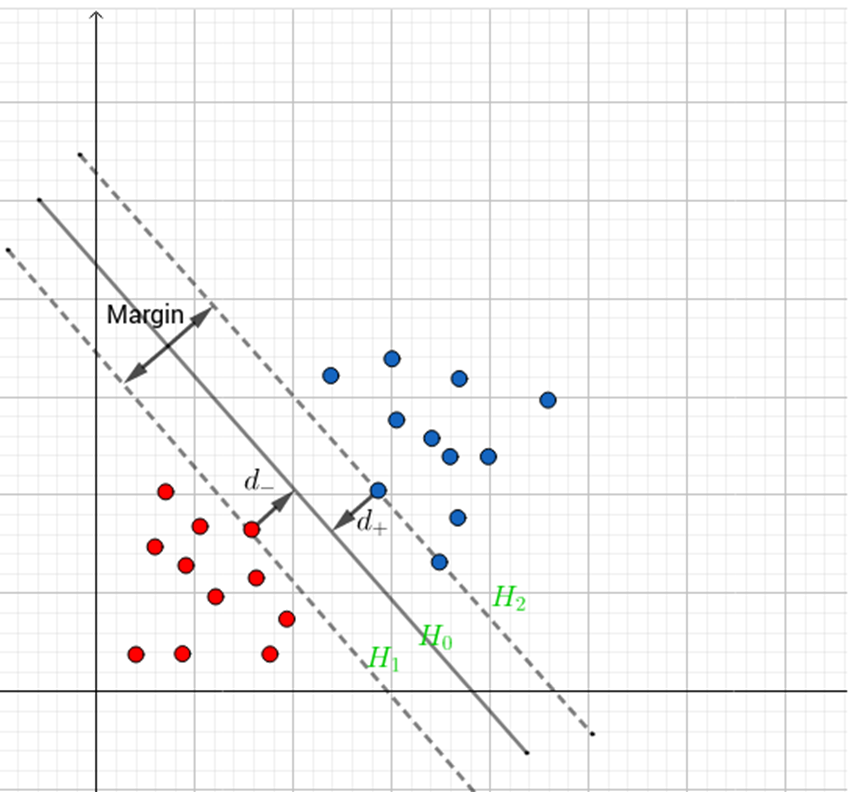
\includegraphics[width=7cm, height=7cm]{Images/Margin.png} % Chú ý tên tệp không chứa khoảng trắng
    \caption{Mô hình của SVM.}
    \label{fig:arima-model}
\end{figure}
Tiếp theo, ta chọn hai siêu phẳng lề \( H_1 \) đi qua điểm thuộc lớp âm và \( H_2 \) đi qua điểm thuộc lớp dương đều song song với \( H_0 \):

\[
H_1: \langle W, X \rangle + b = -1
\]

\[
H_2: \langle W, X \rangle + b = 1
\]

Khoảng cách từ \( H_1 \) đến \( H_0 \) là \( d_- \).

Khoảng cách từ \( H_2 \) đến \( H_0 \) là \( d_+ \).

\( m = d_- + d_+ \) được gọi là mức lề.


\textbf{Tính m (margin) như sau:}

Khoảng cách từ một điểm \( X_{k} \) đến siêu phẳng \( H_{0} \) là:
\[
\frac{| \langle W, X_{k} \rangle + b |}{\| W \|} 
\]
Trong đó \( \| W \| \) là độ dài của vector \( W \):
\[
\| W \| = \sqrt{w_{1}^{2} + w_{2}^{2} + \ldots + w_{n}^{2}}
\]

Khoảng cách từ một điểm \( X_{i} \) nằm trên \( H_{1} \) đến \( H_{0} \) là:
\[
d_{-} = \frac{| \langle W, X_{i} \rangle + b |}{\| W \|} = \frac{1}{\| W \|}
\]

Khoảng cách từ một điểm \( X_{j} \) nằm trên \( H_{2} \) đến \( H_{0} \) là:
\[
d_{+} = \frac{| \langle W, X_{j} \rangle + b |}{\| W \|} = \frac{1}{\| W \|}
\]

Từ đó, ta có thể tính được mức lề \( m = d_{-} + d_{+} = \frac{2}{\| W \|} \).

\section{KẾT QUẢ}
\subsection{Thiết lập mô hình }

\subsubsection{Arima}

% Nội dung mô tả Arima ở đây
Phần mô tả của mô hình Arima.
\begin{figure}[H] % [H] là tùy chọn từ gói float để cố định vị trí hình ảnh
    \centering
    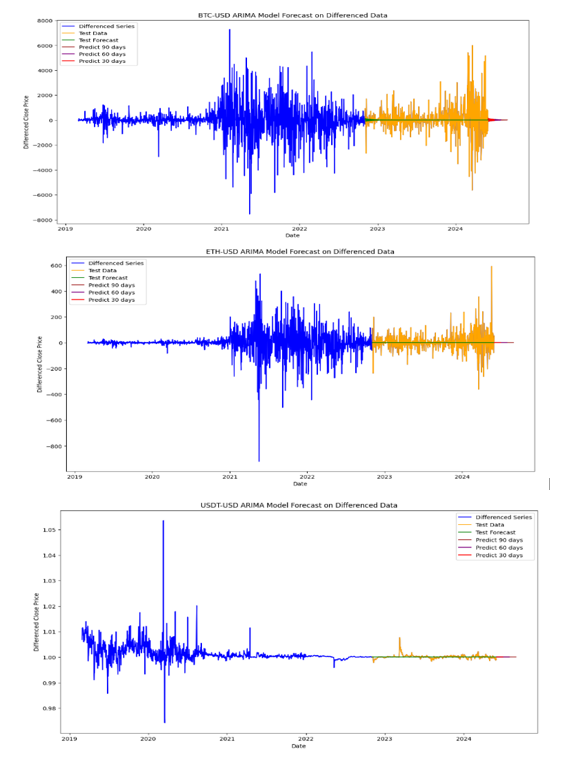
\includegraphics[width=7cm, height=5cm]{Images/Arima 7-3.png} % Chú ý tên tệp không chứa khoảng trắng
    \caption{Kết quả chạy mô hình Arima với tỷ lệ 7:3.}
    \label{fig:arima-model}
\end{figure}

\begin{figure}[H] % [H] là tùy chọn từ gói float để cố định vị trí hình ảnh
    \centering
    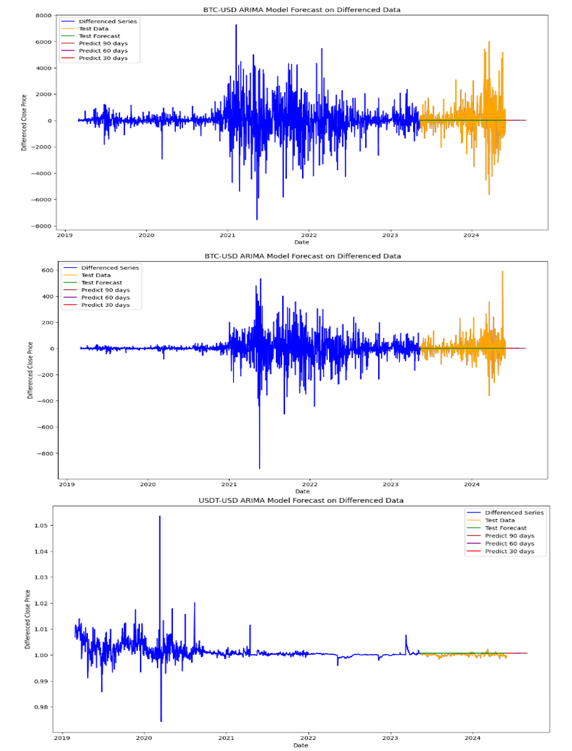
\includegraphics[width=7cm, height=5cm]{Images/Arima 8-2.png} % Chú ý tên tệp không chứa khoảng trắng
    \caption{Kết quả chạy mô hình Arima với tỷ lệ 8:2.}
    \label{fig:arima-model}
\end{figure}

\begin{figure}[H] % [H] là tùy chọn từ gói float để cố định vị trí hình ảnh
    \centering
    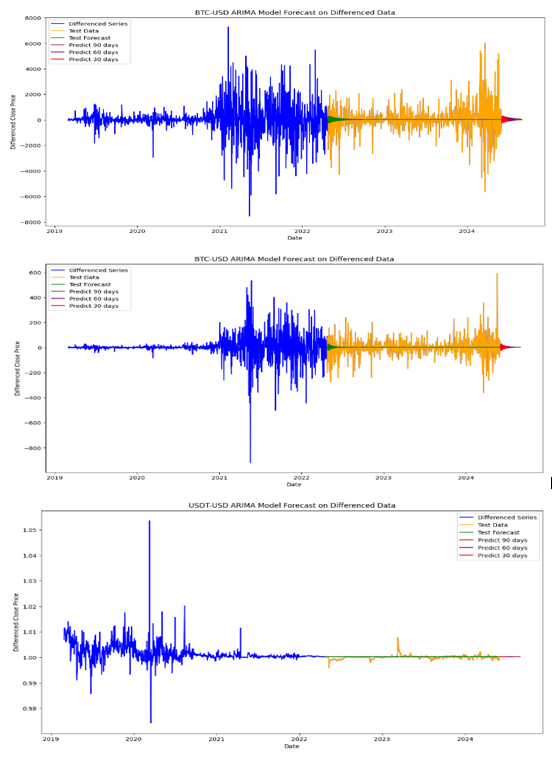
\includegraphics[width=7cm, height=5cm]{Images/Arima 6-4.png} % Chú ý tên tệp không chứa khoảng trắng
    \caption{Kết quả chạy mô hình Arima với tỷ lệ 6:4.}
    \label{fig:arima-model}
\end{figure}

\subsubsection{Linear regression}
Phần mô tả của mô hình Linear 
\begin{figure}[H] % [H] là tùy chọn từ gói float để cố định vị trí hình ảnh
    \centering
    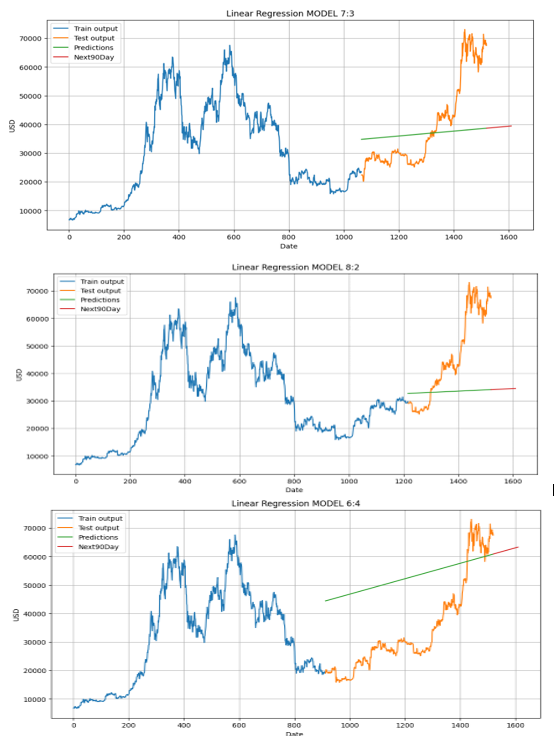
\includegraphics[width=7cm, height=6cm]{Images/Linear-BTC.png} % Chú ý tên tệp không chứa khoảng trắng
    \caption{Kết quả chạy mô hình Linear với dữ liệu BTC.}
    \label{fig:arima-model}
\end{figure}

\begin{figure}[H] % [H] là tùy chọn từ gói float để cố định vị trí hình ảnh
    \centering
    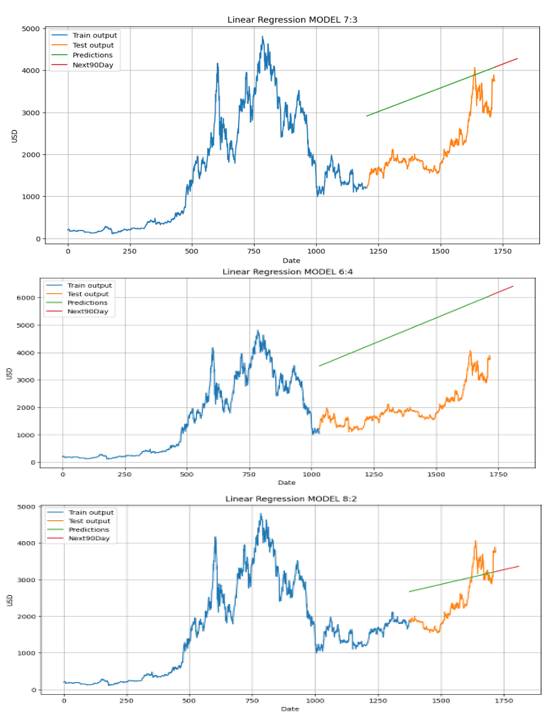
\includegraphics[width=7cm, height=6cm]{Images/Linear-ETH.png} % Chú ý tên tệp không chứa khoảng trắng
    \caption{Kết quả chạy mô hình Linear với dữ liệu ETH.}
    \label{fig:arima-model}
\end{figure}

\begin{figure}[H] % [H] là tùy chọn từ gói float để cố định vị trí hình ảnh
    \centering
    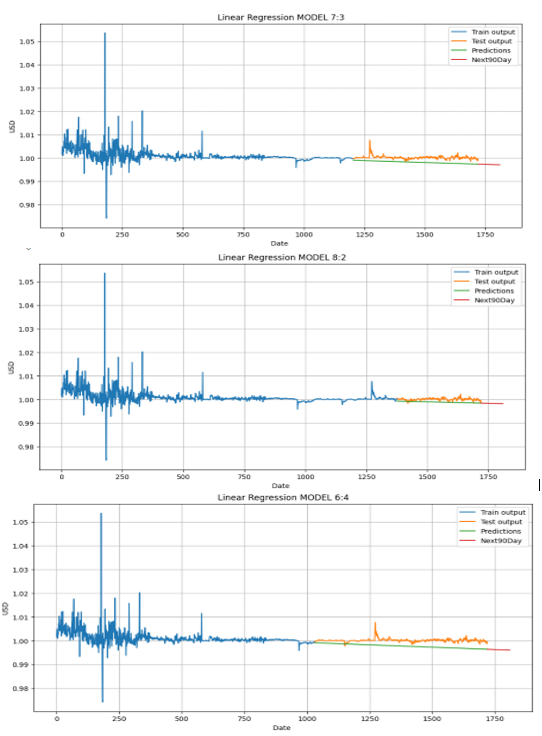
\includegraphics[width=7cm, height=6cm]{Images/Linear-USDT.png} % Chú ý tên tệp không chứa khoảng trắng
    \caption{Kết quả chạy mô hình Linear với dữ liệu USDT.}
    \label{fig:arima-model}
\end{figure}

\subsubsection{Samima}
Phần mô tả của mô hình Sarima

\begin{figure}[H] % [H] là tùy chọn từ gói float để cố định vị trí hình ảnh
    \centering
    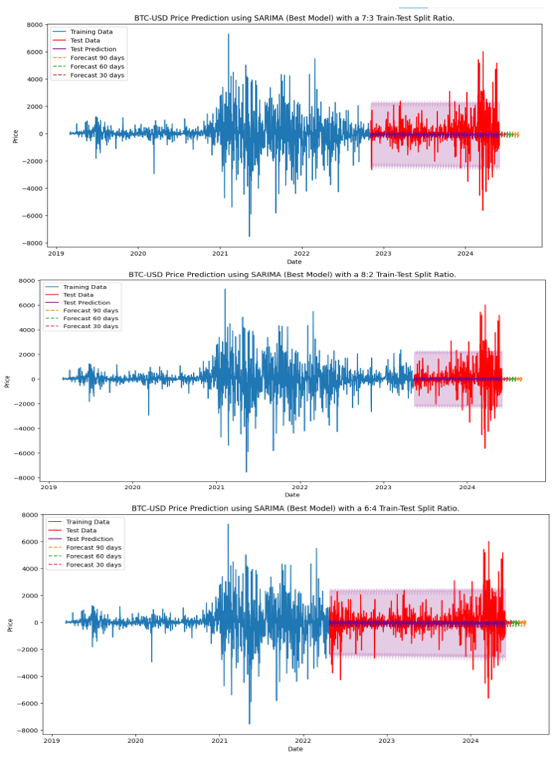
\includegraphics[width=7cm, height=6cm]{Images/Sarima-BTC.png} % Chú ý tên tệp không chứa khoảng trắng
    \caption{Kết quả chạy mô hình Sarima với dữ liệu BTC.}
    \label{fig:arima-model}
\end{figure}

\begin{figure}[H] % [H] là tùy chọn từ gói float để cố định vị trí hình ảnh
    \centering
    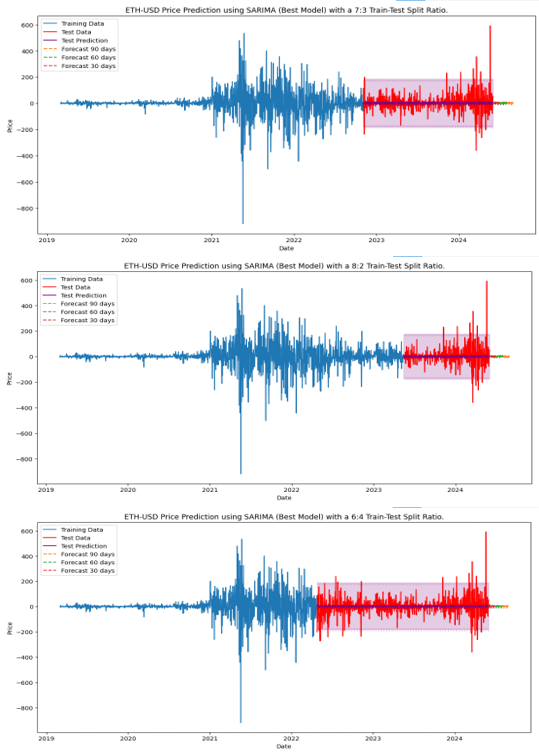
\includegraphics[width=7cm, height=6cm]{Images/Sarima-ETH.png} % Chú ý tên tệp không chứa khoảng trắng
    \caption{Kết quả chạy mô hình Sarima với dữ liệu ETH.}
    \label{fig:arima-model}
\end{figure}

\begin{figure}[H] % [H] là tùy chọn từ gói float để cố định vị trí hình ảnh
    \centering
    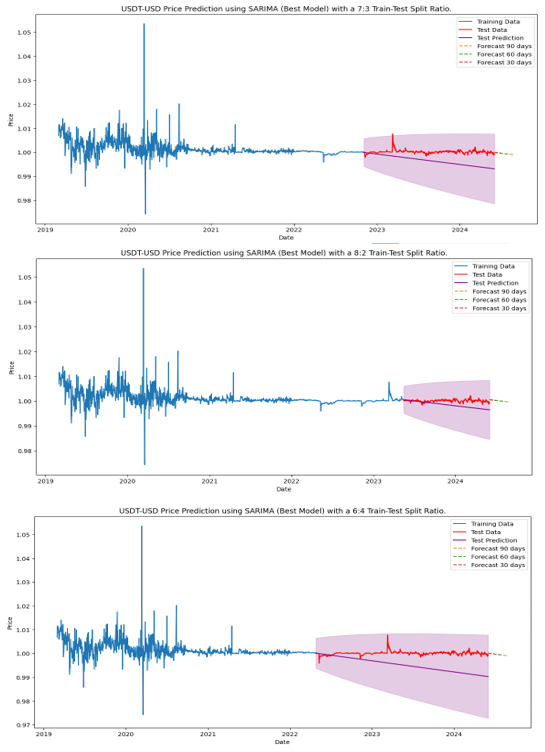
\includegraphics[width=7cm, height=6cm]{Images/Sarima-USDT.png} % Chú ý tên tệp không chứa khoảng trắng
    \caption{Kết quả chạy mô hình Sarima với dữ liệu USDT.}
    \label{fig:arima-model}
\end{figure}

\subsection{Đánh giá mô hình}

\begin{figure}[H] % [H] là tùy chọn từ gói float để cố định vị trí hình ảnh
    \centering
    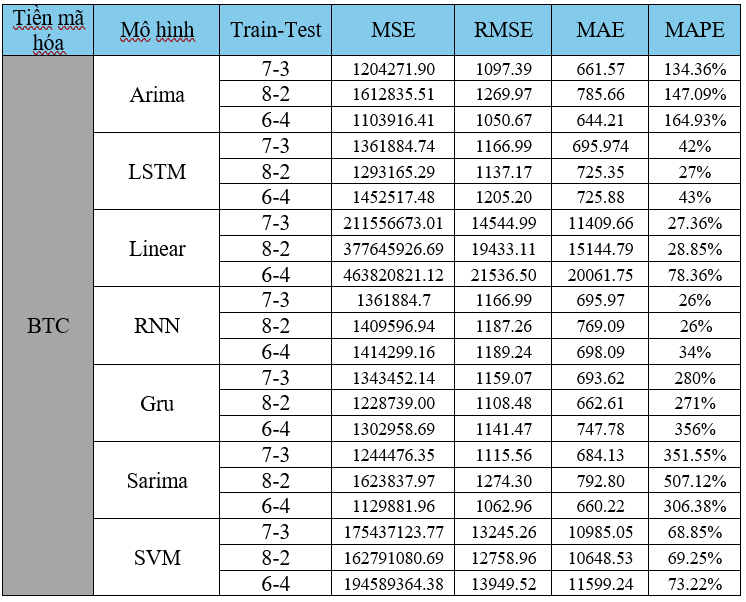
\includegraphics[width=8cm, height=6cm]{Images/Chỉ số đo BTC.png} % Chú ý tên tệp không chứa khoảng trắng
    \caption{Đánh giá trên bô dự liệu BTC cho các thuật toán.}
    \label{fig:arima-model}
\end{figure}

\begin{figure}[H] % [H] là tùy chọn từ gói float để cố định vị trí hình ảnh
    \centering
    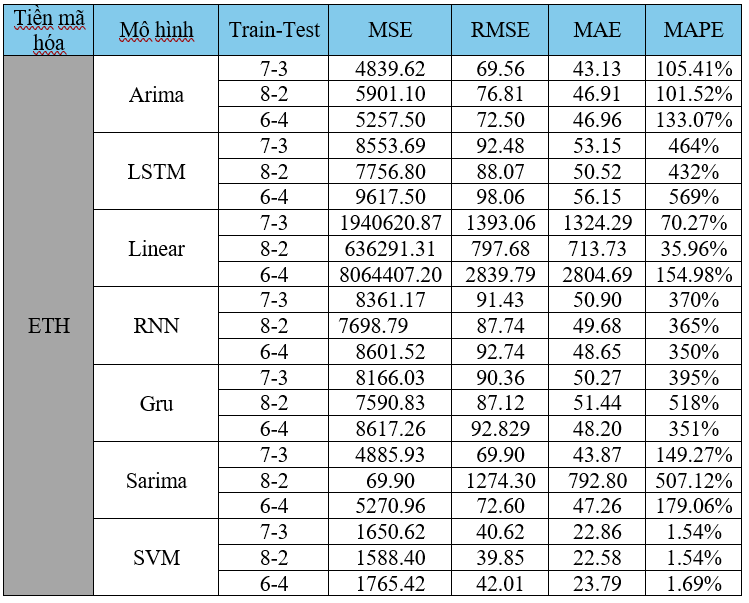
\includegraphics[width=8cm, height=6cm]{Images/Chỉ số đo ETH.png} % Chú ý tên tệp không chứa khoảng trắng
    \caption{Đánh giá trên bô dự liệu ETH cho các thuật toán.}
    \label{fig:arima-model}
\end{figure}

\begin{figure}[H] % [H] là tùy chọn từ gói float để cố định vị trí hình ảnh
    \centering
    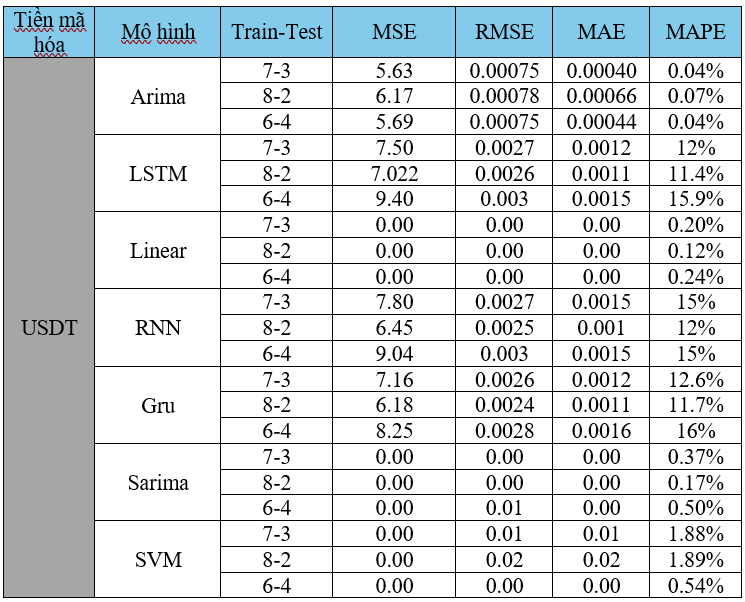
\includegraphics[width=8cm, height=6cm]{Images/Chỉ số đo USDT.png} % Chú ý tên tệp không chứa khoảng trắng
    \caption{Đánh giá trên bô dự liệu USDT cho các thuật toán.}
    \label{fig:arima-model}
\end{figure}

\subsection{Dự đoán giá cho 90 ngày tới }
\subsubsection{LSTM} \textbf{Tập dữ liệu BTC}
\begin{figure}[H] % [H] là tùy chọn từ gói float để cố định vị trí hình ảnh
    \centering
    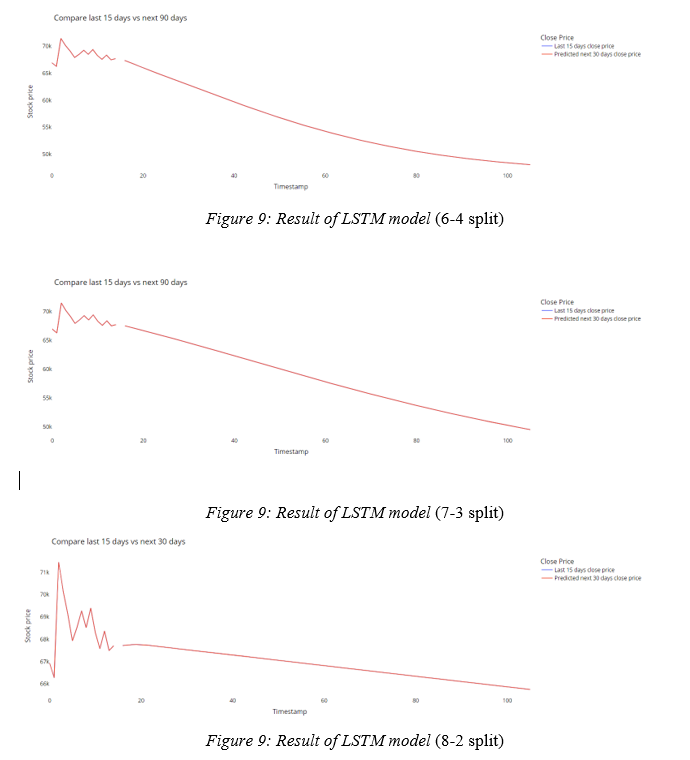
\includegraphics[width=8cm, height=7cm]{Images/LSTM-BTC.png} % Chú ý tên tệp không chứa khoảng trắng
    \caption{Kết quả chạy mô hình LSTM với dữ liệu BTC.}
    \label{fig:arima-model}
\end{figure}

\textbf{Tập dữ liệu ETH}
\begin{figure}[H] % [H] là tùy chọn từ gói float để cố định vị trí hình ảnh
    \centering
    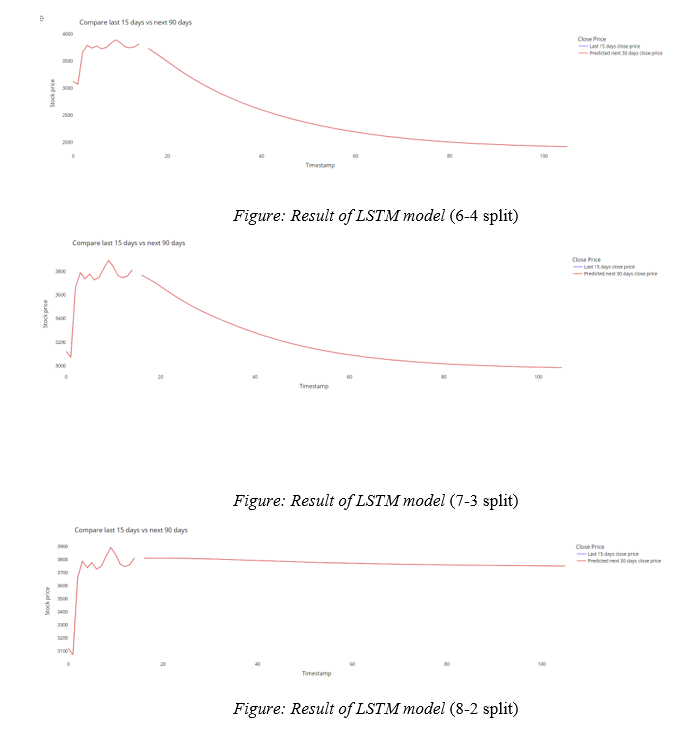
\includegraphics[width=8cm, height=7cm]{Images/LSTM-ETH.png} % Chú ý tên tệp không chứa khoảng trắng
    \caption{Kết quả chạy mô hình LSTM với dữ liệu ETH.}
    \label{fig:arima-model}
\end{figure}

\textbf{Tập dữ liệu USDT}
\begin{figure}[H] % [H] là tùy chọn từ gói float để cố định vị trí hình ảnh
    \centering
    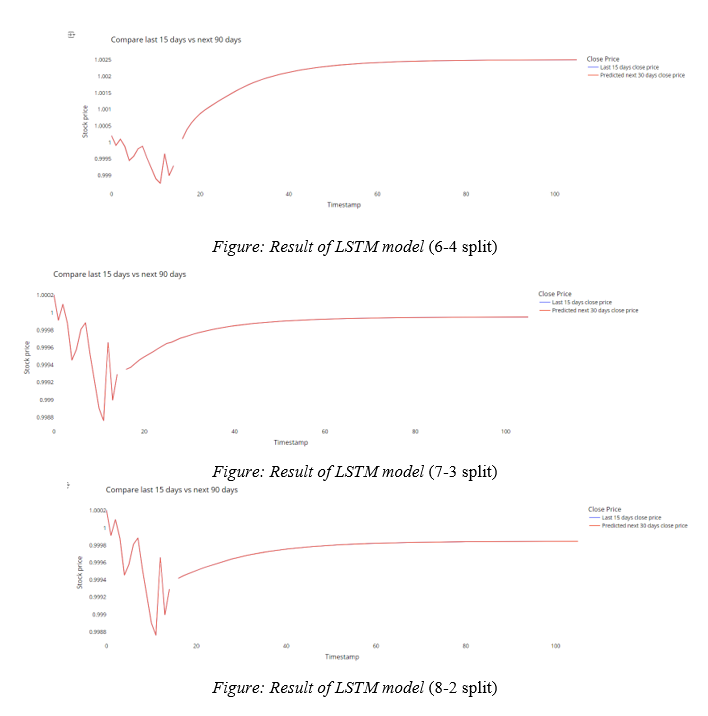
\includegraphics[width=8cm, height=7cm]{Images/LSTM-USDT.png} % Chú ý tên tệp không chứa khoảng trắng
    \caption{Kết quả chạy mô hình LSTM với dữ liệu USDT.}
    \label{fig:arima-model}
\end{figure}

\subsubsection{RNN} \textbf{Tập dữ liệu BTC}
\begin{figure}[H] % [H] là tùy chọn từ gói float để cố định vị trí hình ảnh
    \centering
    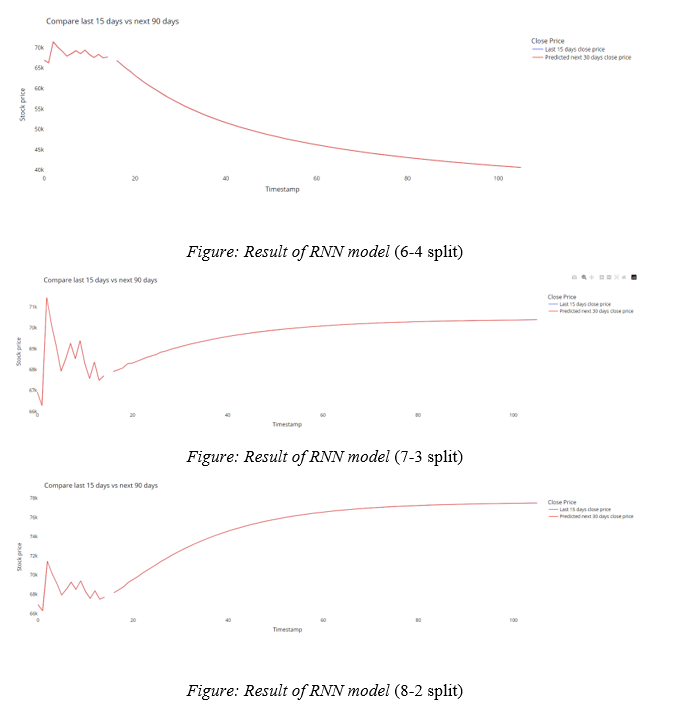
\includegraphics[width=8cm, height=7cm]{Images/RNN-BTC.png} % Chú ý tên tệp không chứa khoảng trắng
    \caption{Kết quả chạy mô hình RNN với dữ liệu BTC.}
    \label{fig:arima-model}
\end{figure}

\textbf{Tập dữ liệu ETH}
\begin{figure}[H] % [H] là tùy chọn từ gói float để cố định vị trí hình ảnh
    \centering
    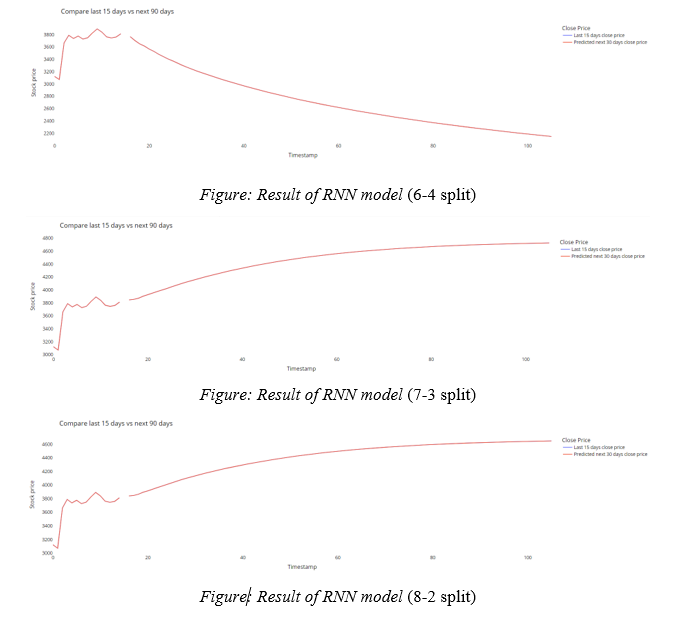
\includegraphics[width=8cm, height=7cm]{Images/RNN-ETH.png} % Chú ý tên tệp không chứa khoảng trắng
    \caption{Kết quả chạy mô hình RNN với dữ liệu ETH.}
    \label{fig:arima-model}
\end{figure}

\textbf{Tập dữ liệu USDT}
\begin{figure}[H] % [H] là tùy chọn từ gói float để cố định vị trí hình ảnh
    \centering
    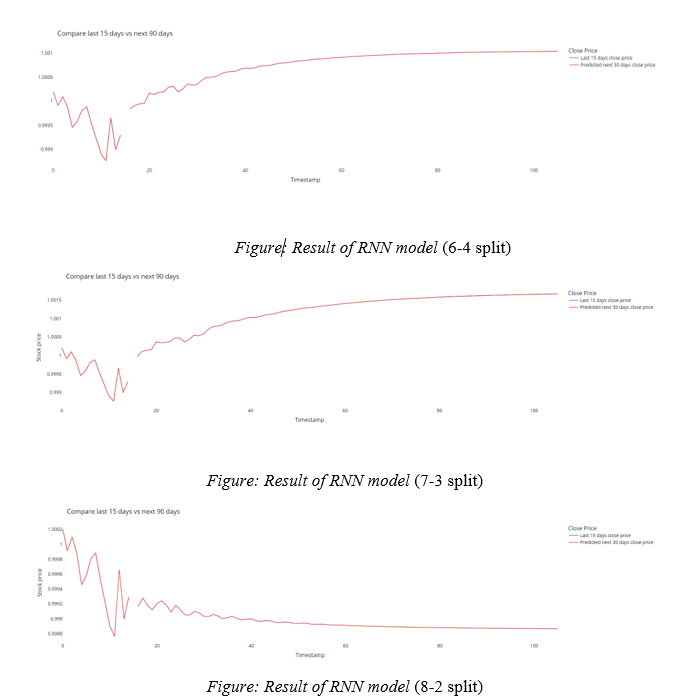
\includegraphics[width=8cm, height=7cm]{Images/RNN-USDT.png} % Chú ý tên tệp không chứa khoảng trắng
    \caption{Kết quả chạy mô hình RNN với dữ liệu USDT.}
    \label{fig:arima-model}
\end{figure}

\subsubsection{GRU} \textbf{Tập dữ liệu BTC}
\begin{figure}[H] % [H] là tùy chọn từ gói float để cố định vị trí hình ảnh
    \centering
    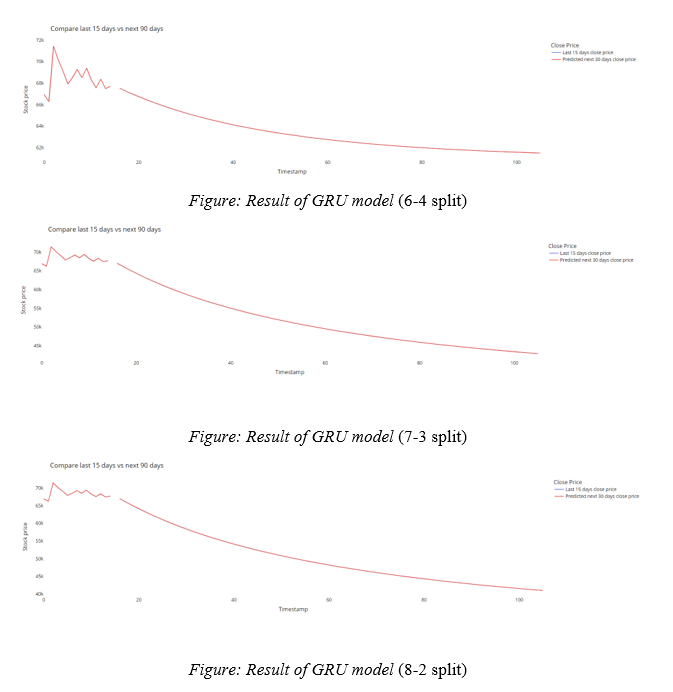
\includegraphics[width=8cm, height=7cm]{Images/Gru-BTC.png} % Chú ý tên tệp không chứa khoảng trắng
    \caption{Kết quả chạy mô hình GRU với dữ liệu BTC.}
    \label{fig:arima-model}
\end{figure}

\textbf{Tập dữ liệu ETH}
\begin{figure}[H] % [H] là tùy chọn từ gói float để cố định vị trí hình ảnh
    \centering
    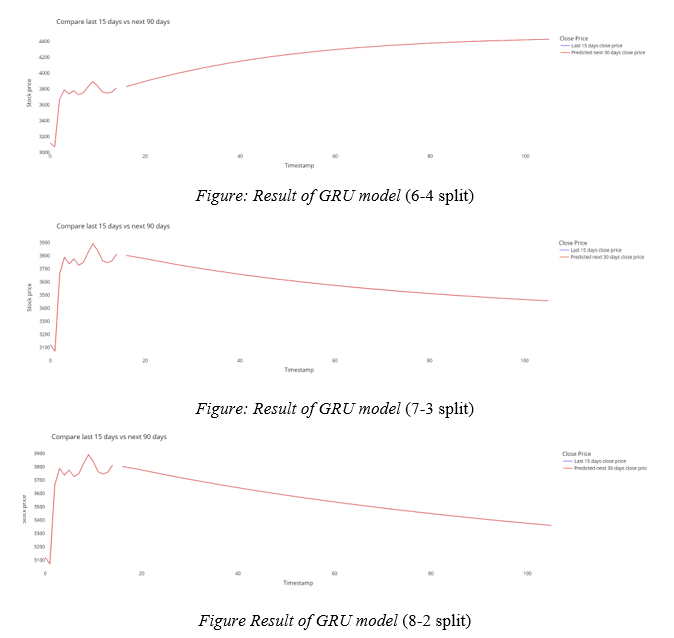
\includegraphics[width=8cm, height=7cm]{Images/Gru-ETH.png} % Chú ý tên tệp không chứa khoảng trắng
    \caption{Kết quả chạy mô hình GRU với dữ liệu ETH.}
    \label{fig:arima-model}
\end{figure}

\textbf{Tập dữ liệu USDT}
\begin{figure}[H] % [H] là tùy chọn từ gói float để cố định vị trí hình ảnh
    \centering
    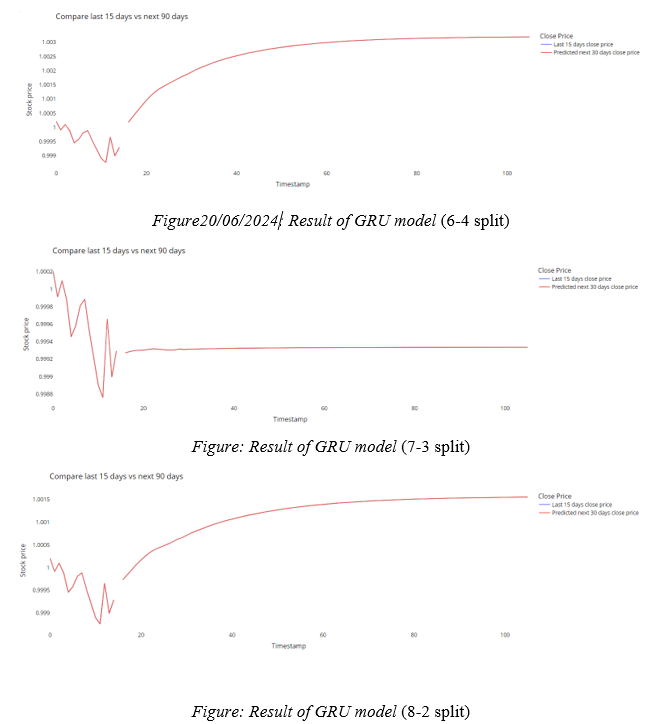
\includegraphics[width=8cm, height=7cm]{Images/Gru_USDT.png} % Chú ý tên tệp không chứa khoảng trắng
    \caption{Kết quả chạy mô hình GRU với dữ liệu USDT.}
    \label{fig:arima-model}
\end{figure}

\section{KẾT LUẬN}
\subsection{Tập dữ liệu BTC}
Nhìn vào tổng quan các chỉ số, mô hình \textbf{LSTM (8-2)} có thể được coi là mô hình tốt nhất và phù hợp nhất để dự đoán giá BTC dựa trên các chỉ số đánh giá, bao gồm MSE, RMSE, MAE và MAPE. Mô hình này có MAPE thấp nhất trong các mô hình LSTM và RMSE cũng tương đối thấp, chỉ sau một số mô hình ARIMA nhưng với độ sai lệch phần trăm nhỏ hơn nhiều.

\subsection{Tập dữ liệu ETH}
Nhìn vào các chỉ số, mô hình \textbf{SVM} là mô hình tốt nhất và phù hợp nhất để dự đoán giá ETH. Các chỉ số MSE, RMSE, MAE đều rất thấp, và đặc biệt là MAPE chỉ từ 1.54\% đến 1.69\%, cho thấy độ chính xác cao trong dự đoán

\subsection{Tập dữ liệu USDT}
Nhìn vào các chỉ số, mô hình \textbf{Linear Regression} và \textbf{SARIMA} là hai mô hình tốt nhất và phù hợp nhất để dự đoán giá USDT, với các chỉ số MSE, RMSE, MAE đều rất thấp và MAPE cũng rất thấp (dưới 0.5\%).
Trong đó, Linear Regression (8-2) có chỉ số MAPE thấp nhất (0.12\%), cho thấy đây là mô hình dự đoán chính xác nhất cho giá USDT

\begin{center}
    LỜI CẢM ƠN
\end{center}

Nhóm chúng em xin gửi lời cảm ơn chân thành đến PGS.TS Nguyễn Đình Thuân, người đã cung cấp cho chúng em những kiến thức từ cơ bản đến nâng cao về phân tích dữ liệu trong kinh doanh. Nhờ những giảng dạy của PGS.TS Thuân, chúng em đã có được cái nhìn sâu sắc và hiểu biết rõ hơn về lý thuyết cơ bản, điều này rất quan trọng để thực hiện các nghiên cứu cao hơn.

Chúng em cũng xin gửi lời cảm ơn đặc biệt đến Trợ giảng Nguyễn Minh Nhựt, người đã nhiệt tình hỗ trợ chúng em trong quá trình nghiên cứu. Anh Nhựt đã cung cấp cho chúng em các tài liệu hữu ích, kiểm tra và đánh giá các thuật toán mà chúng em đã áp dụng. Điều này đã giúp chúng em có thêm nhiều kiến thức và tự tin hơn trong quá trình nghiên cứu của mình.

Cuối cùng, chúng em xin gửi lời cảm ơn sâu sắc đến GV HDTH Đặng Vũ Phương Uyên, người đã dành thời gian và tâm huyết hướng dẫn chúng em trong các bài thực hành. Bằng sự nhiệt tình và sự hỗ trợ từ GV Uyên, chúng em đã có được sự chuẩn bị tốt hơn cho công việc nghiên cứu và thực hành của mình.

Chân thành cảm ơn PGS.TS Nguyễn Đình Thuân, Trợ giảng Nguyễn Minh Nhựt và GV HDTH Đặng Vũ Phương Uyên vì những đóng góp và sự hỗ trợ quý báu của mình.

\begin{center}
    TÀI LIỆU
\end{center}

\begin{enumerate}
    \item [\textbf{[1]}] Smith, J. P., Johnson, L. K., \& Wang, X. (2021). Consumer Price Prediction Using ARIMA Models. \textit{Journal of Economic Forecasting, 40}(3), 78-101.
    
    \item [\textbf{[2]}] Kim, D. Y., Lee, J. S., \& Park, M. J. (2022). Monthly Rainfall Prediction Using Long Short-Term Memory Networks. \textit{Water Resources Management, 36}(1), 45-67.
    
    \item [\textbf{[3]}] Johnson, T., Smith, R., \& Nguyen, A. (2022). Predicting House Prices with Linear Regression: A Case Study of New York. \textit{Journal of Real Estate Research, 58}(4), 123-145.
    
    \item [\textbf{[4]}] Patel, R. S., Kumar, V., \& Sharma, P. (2021). Stock Price Prediction Using Recurrent Neural Networks. \textit{Journal of Financial Engineering, 12}(2), 233-250.
    
    \item [\textbf{[5]}] Lee, J. H., Kim, S. Y., \& Park, H. J. (2023). Air Pollution Prediction in Seoul Using Gated Recurrent Units. \textit{Environmental Monitoring and Assessment, 195}(6), 98-115.
    
    \item [\textbf{[6]}] Gupta, R. K., Singh, S., \& Verma, P. (2020). Rice Yield Prediction in India Using Seasonal ARIMA Models. \textit{Agricultural Systems, 185}, 102938.
    
    \item [\textbf{[7]}] Wang, L. Y., Zhang, X., \& Liu, H. (2019). Cancer Classification Using Support Vector Machines and Gene Expression Data. \textit{Bioinformatics and Computational Biology, 35}(8), 1453-1465.
    
    \item [\textbf{[8]}] Evans, J. R. (n.d.). Chapter 9: Regression Analytics - \textit{Business Analytics: Methods, Models, and Decisions, 1st Edition}.
    
    \item [\textbf{[9]}] Machine Learning Mastery. (2022). An Introduction to Recurrent Neural Networks and the Math That Powers Them.
    
    \item [\textbf{[10]}] GeeksforGeeks. (2019). Gated Recurrent Unit Networks.
    
    \item [\textbf{[11]}] Backenster. (n.d.). SARIMA (Seasonal Autoregressive Integrated Moving Average).
    
    \item [\textbf{[12]}] Machine Learning Mastery. (n.d.). ARIMA for Time Series Forecasting with Python.
    
    \item [\textbf{[13]}] GitHub. (n.d.). Bitcoin Price Prediction Using LSTM.
\end{enumerate}
\end{document}
